\section{Dynamic Resource Allocation in a Manycore OS}\label{eval-dynamic}
%	c.	Dynamic System
%		i.	Single Application � right sizing
%			1.	Without phase changes
%			2.	With phase changes
%			3.	Baseline � all allocations
%			4.	Measure Energy
%		ii.	Video, Animation, and Throughput Applications w/o phase changes
%			1.	Show throughput and missed deadlines for all the possible mixes
%			2.	Is it possible to show optimal?
%			3.	What is the baseline?
%		iii.	Video, Animation, and Throughput Applications w/ phase changes
%			1.	Show throughput and missed deadlines for all the possible mixes
%			2.	Basically just to show the system works

%\cite{tess09,tess_dac}
To evaluate \pacora's ability to make real-time decisions in a real operating system, we implemented it in an in-house research operating system, \tess. We chose to implement in \tess rather than Linux for three reasons:
 \begin{itemize}\itemsep0pt \parskip0pt \parsep5pt
\item \tess is designed around two-level scheduling, meaning it more accurately reflects the system design \pacora assumes
\item \tess allows resource revocation, enabling \pacora to dynamically reallocate resources
\item \tess implements additional resource partitioning and QoS mechanisms, letting \pacora explore allocating more resource types
\end{itemize}
This dynamic framework is used to test our implementations of the algorithms, measure the overhead and reaction times, and illustrate \pacora's ability to work in a real system.

\subsection*{Platform}
Our dynamic experiments are all run on an Intel Nehalem-EP system with two 2.66-GHz Xeon X5550 quad-core processors and hyperthreading enabled with 16 hardware threads. Tis system also contains a 1-Gbps Intel Pro/1000 Ethernet network adapter.
\tess allocates resources directly to applications, and the applications employ a second-level scheduler to schedule work onto the resources.  There are two scheduling frameworks available in \tess: a cooperative framework called Lithe (LIquid THrEads)~\cite{lithe} and a preemptive one called PULSE (Preemptive User-Level SchEduling).  All of our experiments use PULSE, with two different scheduling strategies: applications with responsiveness requirements use an earliest-deadline-first (EDF) scheduler and throughput-oriented applications use a global-round-robin (GRR) scheduler.

In addition to allocating cores and cache ways as with our static framework, \tess can also allocate fractions of network bandwidth.  In our experiments, we show \pacora allocating cores and network bandwidth because the experimental platform, which has the advantage of more cores, does not have cache partitioning.  We have also experimented with additional resources such as memory pages and cpu utilization, but the results are not presented here.

\subsection*{Performance and Energy Measurement}
Applications report their own measured response times to \pacora through a message-passing interface built into \tess.  \pacora uses this information to build models, and we also use this information to show if the application is making its deadlines for the experiments.

\tess enables \pacora to directly measure the system energy.  However, energy counters are not available on our Nehalem-EP system and thus we extend the power model from the Sandy Bridge system to function as our Application 0 RTF.

\subsection*{Description of Workloads}
Our workload is designed to represent the scenario of a video conference, where each participant requires a separate, performance guaranteed video stream.
New participants may join the conference and others may leave, increasing or decreasing the number of streams running at any given time.  Additionally, the speaker's video is larger and has higher resolution than the other video streams, and as the speaker changes the requirements for the video streams change. While conferencing, compute-intensive tasks such as virus scans or file indexing could be executed in the background.

Our streaming video application is a multi-threaded, CPU- and network-intensive workload intended to simulate video chat applications like Skype and Facetime.
Each video stream is encoded offline in the H.264 format using libx264, transported across the network through a TCP connection, and decoded and displayed by the \tess client. The client receives, decodes and displays each frame using libffmpeg and libx264. Each video stream has a corresponding EDF-scheduled thread with 33 ms deadlines using our second-level EDF scheduler.

We use psearchy~\cite{psearchy}, a parallel text indexer, from MOSBENCH\cite{mosbench} as our file indexing application. We also use a network bandwidth hog application designed to contend with the video player for bandwidth by constantly sending UDP messages to the Linux box.

\subsection*{Resource Allocation Experiments}
\begin{figure*}[!t]
	\begin{center}	
%		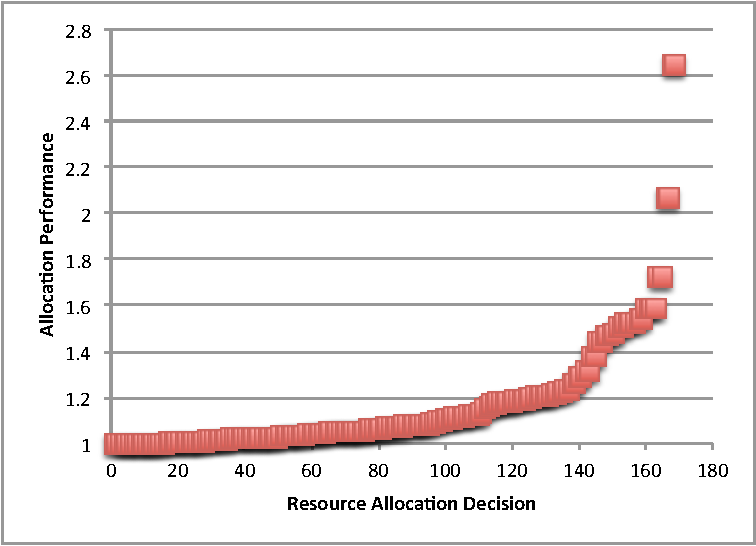
\includegraphics[width=.45\textwidth]{parsec_decision_points.pdf}
		\caption{Resource Allocations of video conferencing through time as participants enter and leave and the video in focus changes with the computer operating in wall power mode}
		\label{video_experiment_wp}
	\end{center}
\end{figure*}

\begin{figure*}[!t]
	\begin{center}	
%		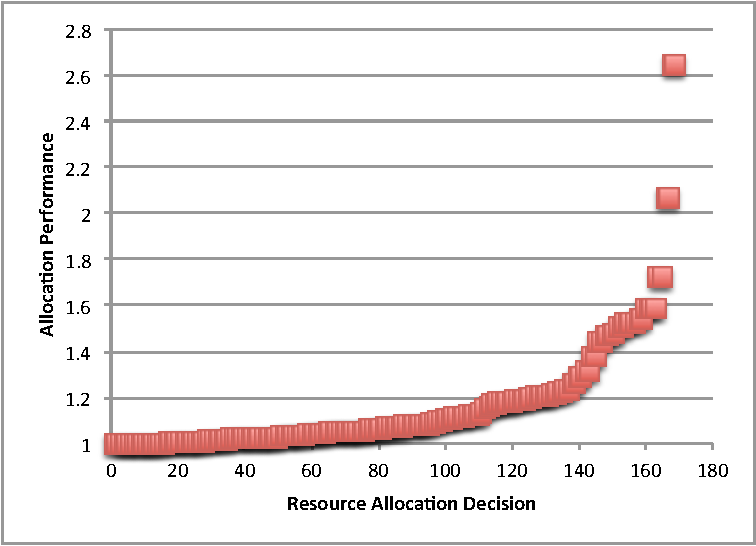
\includegraphics[width=.45\textwidth]{parsec_decision_points.pdf}
		\caption{Resource Allocations of video conferencing through time as participants enter and leave and the video in focus changes with the computer operating in battery power mode}
		\label{video_experiment_battery}
	\end{center}
\end{figure*}

Figure~\ref{video_experiment_wp} shows the resource allocations for our video conference scenario when the computer is using wall power. Figure~\ref{video_experiment_battery} shows same scenario except the computer is now using battery power and thus we have increased the importance of application 0.








